
\section{Шинжилгээ }
\subsection{Үйл ажиллагааны диаграм}
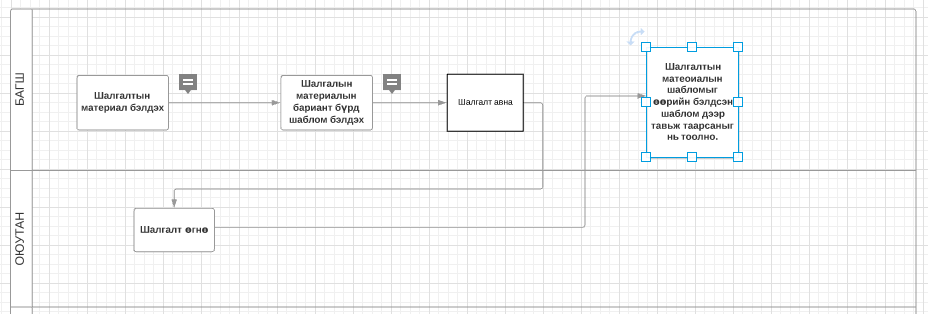
\includegraphics[width=15cm,height=6cm, scale=0.5]{Figures/ac1.png}
\hspace*{0pt}\hfill Багш шаблом урьчилан бэлдэж шалгалт авах үйл ажиллагааны диаграм.
\newline
\newline

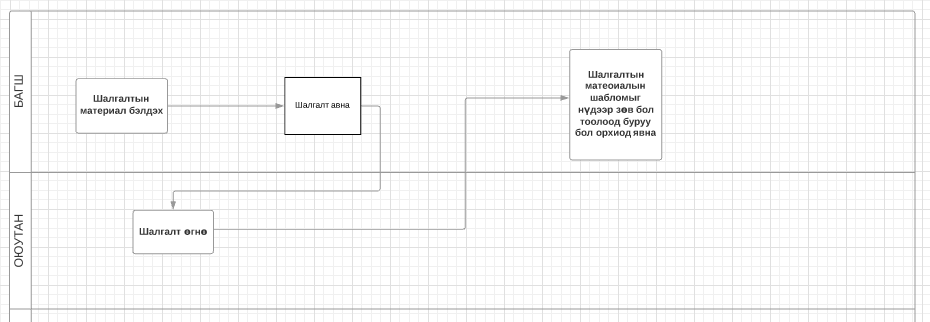
\includegraphics[width=15cm,height=6cm, scale=0.5]{Figures/ac2.png}
\hspace*{0pt}\hfill Багш шаблом урьчилан бэлдээгүй шалгалт авах үйл ажиллагааны диаграм.
\newline
\subsection{Функциональ шаардлага}
\begin{flushleft}
- Нэвтрэх
\linebreak
- Асуулт бүртгэх
\linebreak
- Хариулт бүртгэх
\linebreak
- Шалгалт бүртгэх\linebreak
- Асуултын жагсаалт харах\linebreak
- Шалгалтын үр дүнгийн тайлан харах.\linebreak
- Шалгалт өгсөн оюутнуудын тоогоор тайлан харах.\linebreak
\end{flushleft}
\subsection{Функциональ бус шаардлага}
\begin{flushleft}
- Шалгалтын асуултууд бүгд давхардахгүй дараалалтай шалгалтууд хэвлэгдэнэ.\linebreak
- Шалгалтын ID болон Оюутны ID-г шабломноос авна.\linebreak
- Оюутны шалгалтын оноог бааз руу хуулна.\linebreak
- Шалгалтын асуултууд дээр дүн шинжилгээ хийнэ.\linebreak
\end{flushleft}
